\documentclass{article}



\usepackage{fullpage}
\usepackage{nopageno}
\usepackage{amsmath}
\usepackage{amsfonts}
\usepackage{graphicx}
\usepackage{framed}
\usepackage{xcolor}

\definecolor{dark_red}{rgb}{0.5,0.0,0.0}
\definecolor{dark_green}{rgb}{0.0,0.5,0.0}
\definecolor{dark_blue}{rgb}{0.0,0.0,0.5}

\newcommand{\dr}[1]{\textcolor{dark_red}{#1}}
\newcommand{\dg}[1]{\textcolor{dark_green}{#1}}
\newcommand{\db}[1]{\textcolor{dark_blue}{#1}}


\begin{document}

\section*{Polar Coordinates}

\begin{tabular}{cc}
\parbox{0.5\textwidth}{
As an alternative to Cartesian coordinates, polar coordinates provide another means of quantifying the position of a point using two numbers. Polar coordinates describe a point \(P\)'s location using a pair of numbers \((r, \theta)\) instead of \((x, y)\). \(r\) denotes the ``distance" of \(P\) from the origin, while \(\theta\) denotes the counterclockwise rotation from the positive \(x\)-axis required to aim at point \(P\). Polar coordinates are illustrated by the image on the right.
\begin{itemize}
\item \(\theta\) will always be measured in radians. 
\item The rotation \(\theta\) is always measured relative to the positive \(x\)-axis.
\item A clockwise rotation corresponds to a negative value of \(\theta\).
\end{itemize} 
} & \parbox{0.5\textwidth}{
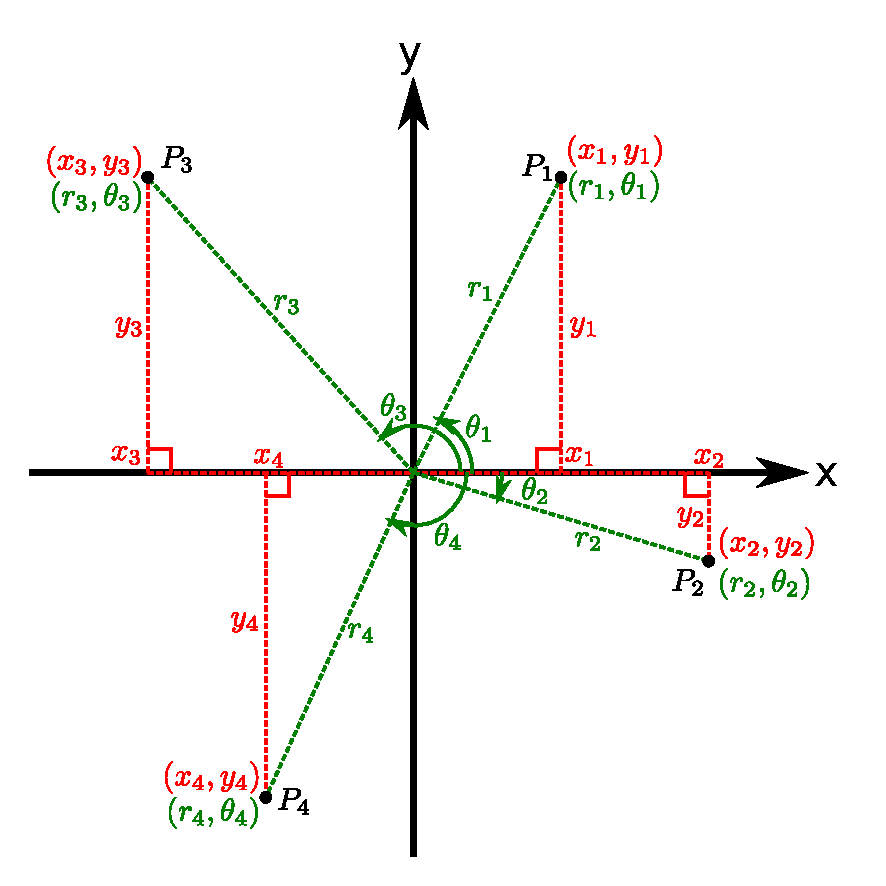
\includegraphics[width = 0.5\textwidth]{cartesian_vs_polar_coordinates}
}
\end{tabular}

\begin{tabular}{cc}
\parbox{0.5\textwidth}{
Despite \(r\) denoting the ``distance" required to reach point \(P\), \(r\) can still be negative. Initially facing in the direction of the positive \(x\)-axis, coordinate \(\theta\) denotes the counterclockwise rotation required to lineup point \(P\). \(r\) is positive if forwards movement is necessary to reach point \(P\), while \(r\) is {\bf negative} if {\bf backwards} movement is required to reach point \(P\).
} & \parbox{0.5\textwidth}{
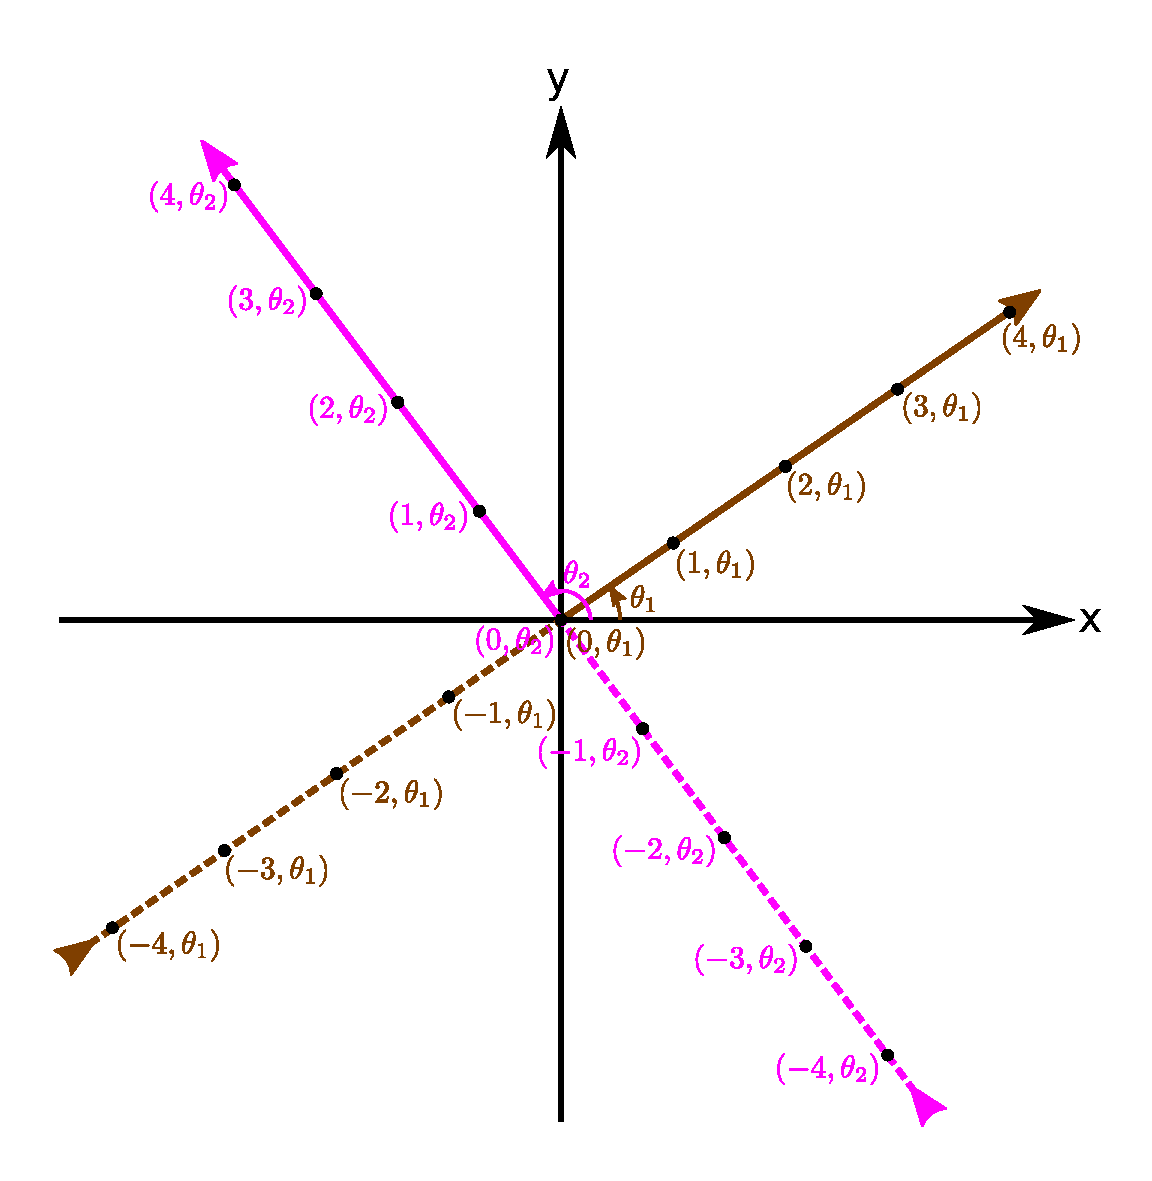
\includegraphics[width = 0.5\textwidth]{negative_r}
}
\end{tabular}


Given polar coordinate \((r, \theta)\), for every integer \(k \in \mathbb{Z}\), the polar coordinates \((r, \theta + k \cdot 2\pi) = (r, \theta + 2 k \pi)\) and \((-r, \theta + \pi + k \cdot 2\pi) = (-r, \theta + (2k + 1)\pi)\) describe the same point \((r, \theta)\). Adding or subtracting full revolutions from \(\theta\) does not change the referenced point. In addition, adding or subtracting a half revolution followed by sign change of \(r\) does not change the referenced point.

In polar coordinates, 
\[\cdots = (-r, \theta - 3\pi) = (r, \theta - 2\pi) = (-r, \theta - \pi) = (r, \theta) = (-r, \theta + \pi) = (r, \theta + 2\pi) = (-r, \theta + 3\pi) = \cdots\]
all denote the same point. 

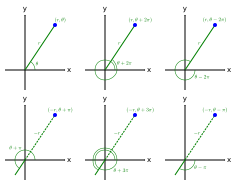
\includegraphics[scale = 0.65]{multiple_polar_coordinates}

\textbf{Examples:}
\begin{itemize}
\item The polar coordinates \((3, 3\pi/4)\), \((3, 11\pi/4)\), \((3, -5\pi/4)\), \((-3, 7\pi/4)\), \((-3, 15\pi/4)\), and \((-3, -\pi/4)\) all describe the same point.
\end{itemize}



\subsection*{Polar coordinates and the trigonometric ratios}

In the image below, the red unit circle, the green tangent line defined by \(x = 1\), and the blue tangent line defined by \(y = 1\) are shown. Starting from the positive \(x\) axis, rotate by a counterclockwise angle of \(\theta\). A ray projected forwards corresponds to positive values of \(r\). A ray projected backwards corresponds to negative values of \(r\). The positive ray intersects the unit circle at the point with Cartesian coordinates \((\cos\theta, \sin\theta)\), which also has the polar coordinates \((1, \theta)\). The rays intersect the green tangent line at the point with Cartesian coordinates \((1, \tan\theta)\), which also has the polar coordinates \((\sec\theta, \theta)\). The rays intersect the blue tangent line at the point with Cartesian coordinates \((\cot\theta, 1)\), which also has the polar coordinates \((\csc\theta, \theta)\). These points are depicted in the image below for two different values of \(\theta\), namely \(\theta_1\) and \(\theta_2\). \(\theta_1\) is chosen from the interval \((0,\pi/2)\) and generates the brown rays, while \(\theta_2\) is chosen from the interval \((\pi/2,\pi)\) and generates the pink rays.

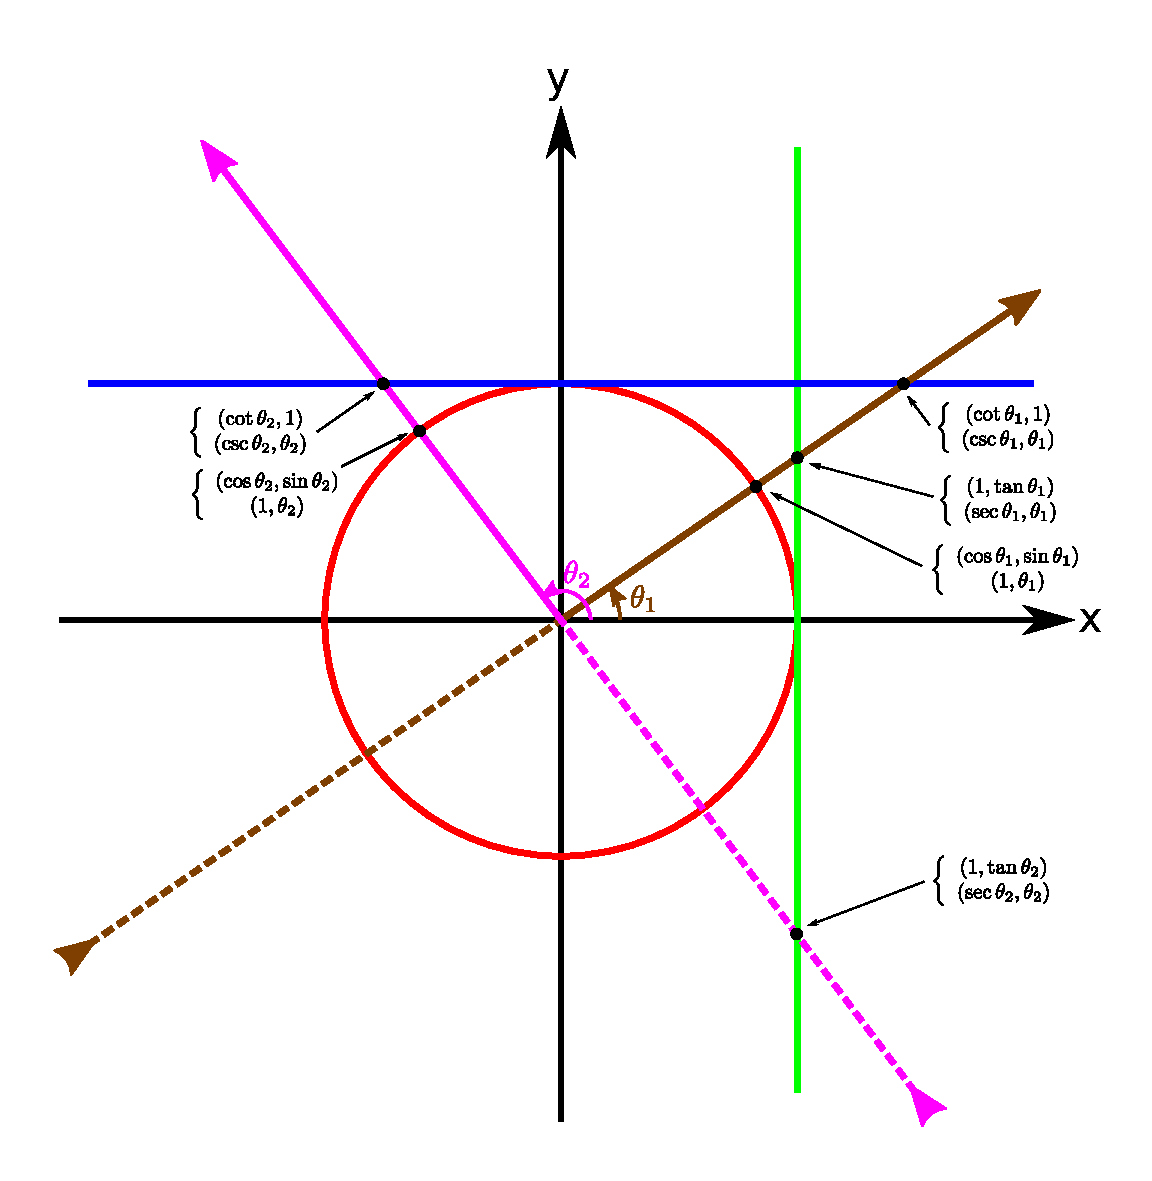
\includegraphics[scale = 0.9]{the_unit_circle_and_polar_coordinates}




\subsection*{Polar to Cartesian conversion}

\begin{tabular}{cc}
\parbox{0.5\textwidth}{
Given an arbitrary polar coordinate \((r, \theta)\), there is only one Cartesian coordinate \((x, y)\) for the point generated by \((r, \theta)\). Project the ray rotated a counterclockwise angle of \(\theta\) from the positive \(x\)-axis. This ray intersects the unit circle at a point with Cartesian coordinates \((\cos\theta, \sin\theta)\) and polar coordinates \((1, \theta)\). Scaling every length uniformly by \(r\) changes the Cartesian coordinate to \((r\cos\theta, r\sin\theta)\) and the polar coordinate to \((r, \theta)\). Therefore:
\[\left\{\begin{array}{c} x = r\cos\theta \\ y = r\sin\theta \end{array}\right.\]
is how the polar coordinate \((r, \theta)\) is converted to Cartesian coordinate \((x, y)\).
} & \parbox{0.5\textwidth}{
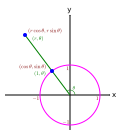
\includegraphics[width = 0.5\textwidth]{polar_to_cartesian_conversion}
}
\end{tabular}

\textbf{Examples:}
\begin{itemize}
\item The polar coordinate \((r, \theta) = (3, \pi/5)\) converted to a Cartesian coordinate is \((x, y) = (3\cos(\pi/5), 3\sin(\pi/5)) \approx (2.42705, 1.76336)\)
\item The polar coordinate \((r, \theta) = (7, 0.77\pi)\) converted to a Cartesian coordinate is \((x, y) = (7\cos(0.77\pi), 7\sin(0.77\pi)) \approx (-5.25078, 4.62918)\)
\item The polar coordinate \((r, \theta) = (2.6, -1.67\pi)\) converted to a Cartesian coordinate is \\ \((x, y) = (2.6\cos(-1.67\pi), 2.6\sin(-1.67\pi)) \approx (1.32351, 2.23793)\)
\item The polar coordinate \((r, \theta) = (2.6, 0.33\pi)\) converted to a Cartesian coordinate is \\ \((x, y) = (2.6\cos(0.33\pi), 2.6\sin(0.33\pi)) \approx (1.32351, 2.23793)\)
\item The polar coordinate \((r, \theta) = (-3, \pi/5)\) converted to a Cartesian coordinate is \((x, y) = (-3\cos(\pi/5), -3\sin(\pi/5)) \approx (-2.42705, -1.76336)\)
\end{itemize}




\subsection*{Cartesian to polar conversion}

Given an arbitrary Cartesian coordinate \((x, y)\), a polar coordinate \((r, \theta)\) that generates the same point as \((x, y)\) is sought.

There are infinitely many choices of polar coordinate \((r,\theta)\) for the given Cartesian coordinate \((x,y)\). To limit our choices down to one alternative, the following restrictions will be placed on \(r\) and \(\theta\):
\[\left\{\begin{array}{c} r \geq 0 \\ (r = 0) \implies (\theta = 0) \\ -\pi < \theta \leq \pi \end{array}\right.\] 
\begin{itemize}
\item Since \(r \geq 0\), only non-negative choices of \(r\) will be considered, so \(r\) is simply the distance that the point \((x,y)\) is from the origin: \(r = \sqrt{x^2 + y^2}\). 
\item The condition \((r = 0) \implies (\theta = 0)\) means that \(\theta = 0\) if \(r = 0\), which means that the \(\theta\) coordinate of the origin point, which could have been any value, is defaulted to \(\theta = 0\). 
\item The condition \(-\pi < \theta \leq \pi\) means that a counterclockwise twist is used to reach points above the \(x\)-axis, and a clockwise twist is used to reach points beneath the \(x\)-axis. Moreover, a twist of \(\pi\) (which is counterclockwise) is used to reach the negative \(x\)-axis.
\end{itemize}

It is clear that \(r\) is simply the distance that the point \((x,y)\) is from the origin: \(r = \sqrt{x^2 + y^2}\). Computing \(\theta\) is a more difficult task. 

To find \(\theta\), consider the line segment that connects the origin to point \((x, y)\). The counterclockwise angle that this line segment makes with the positive \(x\)-axis is \(\theta\). Extrapolating this line segment to a line, this line will intersect the vertical line defined by \(x = 1\) at the Cartesian point \((1, y/x)\). This is because the line segment has a slope of \(y/x\), so the change in \(y\) over a unit change in \(x\) is \(y/x\). {\bf Use the image below for illustration.} Given a line that makes a counterclockwise angle of \(\theta\) with the \(x\)-axis, this line intersects the line \(x = 1\) at the Cartesian point \((1, \tan\theta)\) (revisit the discussions related to the unit circle). Since \((1, y/x)\) and \((1, \tan\theta)\) are the same point, \(\tan\theta = y/x\). 

The fact that \(\tan\theta = y/x\) can also be established from \(x = r\cos\theta\) and \(y = r\sin\theta\):
\[\frac{y}{x} = \frac{r\sin\theta}{r\cos\theta} = \frac{\sin\theta}{\cos\theta} = \tan\theta\]

In the image below, it can be seen that if \(x > 0\), then \(\theta = \tan^{-1}(y/x)\), whereas if \(x < 0\), then a half rotation needs to be either added to or subtracted from \(\tan^{-1}(y/x)\) to get \(\theta\). 

In the case where \(x < 0\), 
\begin{itemize}
\item If \(y/x \leq 0\), then the range of values of \(\tan^{-1}(y/x)\) is \((-\pi/2, 0]\), so a half rotation must be added to give values of \(\theta\) from the range \((\pi/2, \pi]\) which is a valid subset of the target range \((-\pi, \pi]\). This can be seen with point \((x_3, y_3)\) in the image, where a half rotation needs to be added to \(\tan^{-1}(y_3/x_3)\) to get \(\theta_3\).
\item If \(y/x > 0\), then the range of values of \(\tan^{-1}(y/x)\) is \((0, \pi/2)\), so a half rotation must be subtracted to give values of \(\theta\) from the range \((-\pi, -\pi/2)\) which is a valid subset of the target range \((-\pi, \pi]\). This can be seen with point \((x_4, y_4)\) in the image, where a half rotation needs to be subtracted from \(\tan^{-1}(y_4/x_4)\) to get \(\theta_4\).
\end{itemize}

In summary, 
\begin{itemize}
\item If \(x > 0\), then \(\theta = \tan^{-1}(y/x)\)
\item If \(x = 0\), then
	\begin{itemize}
	\item[*] If \(y > 0\), then \(\theta = \pi/2\)
	\item[*] If \(y = 0\), then \(\theta = 0\) (this is the origin point)
	\item[*] If \(y < 0\), then \(\theta = -\pi/2\)
	\end{itemize}
\item If \(x < 0\), then
	\begin{itemize}
	\item[*] If \(y \geq 0\), then \(\theta = \tan^{-1}(y/x) + \pi\)
	\item[*] If \(y < 0\), then \(\theta = \tan^{-1}(y/x) - \pi\)
	\end{itemize}
\end{itemize}

%From the information \(\tan\theta = y/x\), there are an infinite number of values for \(\theta\) that satisfy this equation. Restricting \(\theta\) to the interval \((-\pi, \pi]\) narrows the possible solutions down to 2 alternatives. When \(y/x > 0\), the candidate values of \(\theta\) are \(\tan^{-1}(y/x)\)

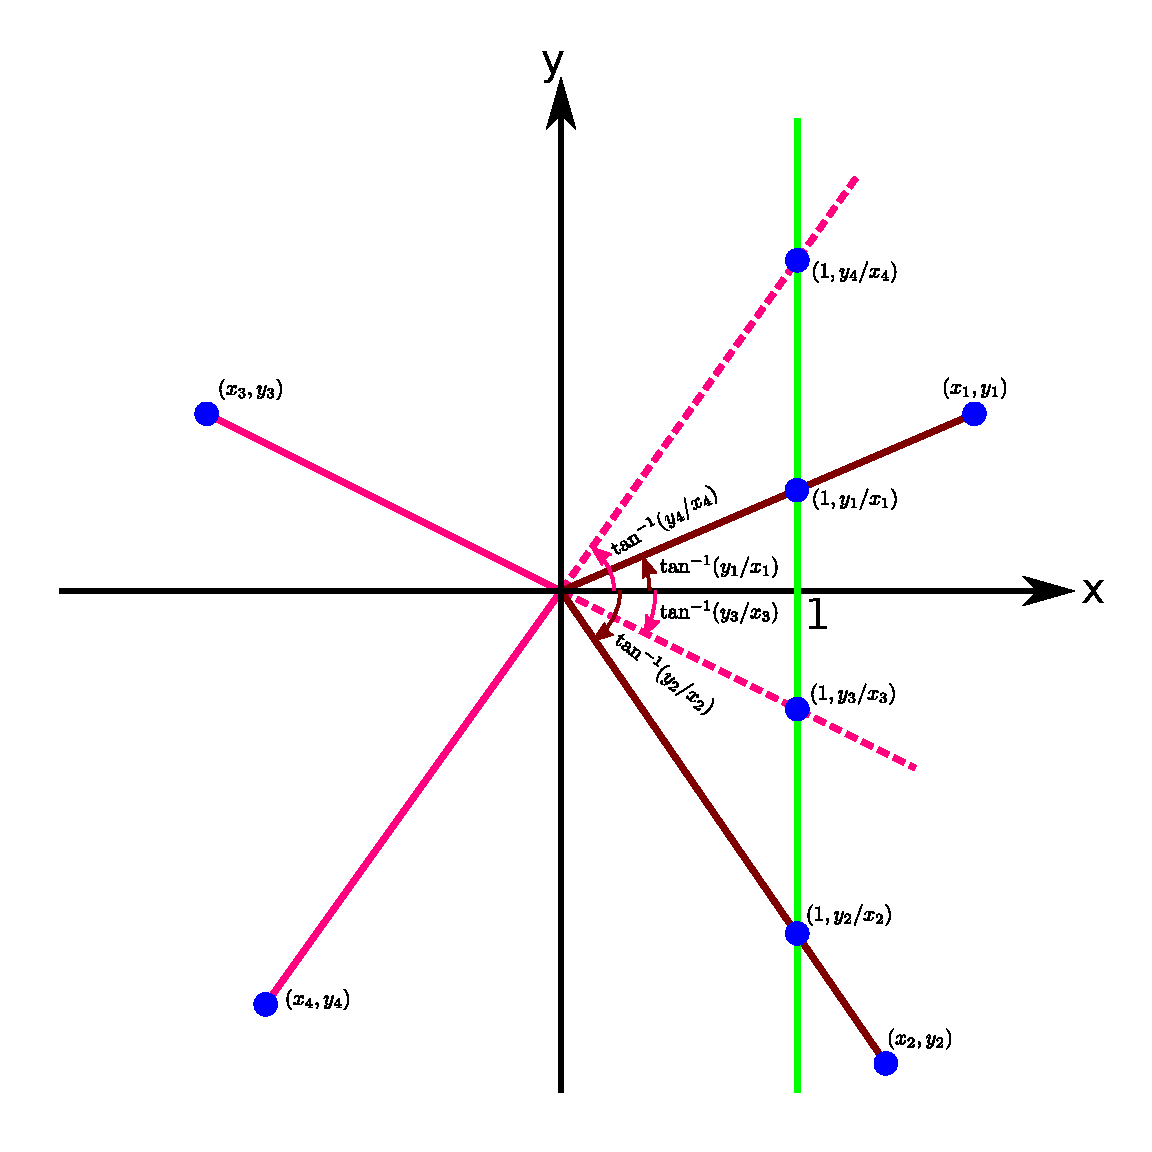
\includegraphics[scale = 0.9]{computing_theta}


\textbf{Examples:}
\begin{itemize}
\item The Cartesian coordinate \((x, y) = (1, 2)\) converted to a polar coordinate gives \(r = \sqrt{1^2 + 2^2} \approx 2.23607\) and \(\theta = \tan^{-1}(2/1) \approx 1.10715\). Hence \((r, \theta) \approx (2.23607, 1.10715)\) is one possible choice of polar coordinate. 
\item The Cartesian coordinate \((x, y) = (4, -3)\) converted to a polar coordinate gives \(r = \sqrt{4^2 + (-3)^2} = 5\) and \(\theta = \tan^{-1}((-3)/4) \approx -0.643501\). Hence \((r, \theta) \approx (5, -0.643501)\) is one possible choice of polar coordinate. 
\item The Cartesian coordinate \((x, y) = (0, 6)\) converted to a polar coordinate gives \(r = \sqrt{0^2 + 6^2} = 6\) and \(\theta = \pi/2 \approx 1.57080\). Hence \((r, \theta) \approx (6, 1.57080)\) is one possible choice of polar coordinate.  
\item The Cartesian coordinate \((x, y) = (0, 0)\) converted to a polar coordinate gives \(r = \sqrt{0^2 + 0^2} = 0\) and \(\theta = 0\). Hence \((r, \theta) = (0, 0)\) is one possible choice of polar coordinate.
\item The Cartesian coordinate \((x, y) = (0, -3)\) converted to a polar coordinate gives \(r = \sqrt{0^2 + (-3)^2} = 3\) and \(\theta = -\pi/2 \approx -1.57080\). Hence \((r, \theta) \approx (3, -1.57080)\) is one possible choice of polar coordinate.
\item The Cartesian coordinate \((x, y) = (-2, 5)\) converted to a polar coordinate gives \(r = \sqrt{(-2)^2 + 5^2} \approx 5.38516\) and \(\theta = \tan^{-1}(5/(-2)) + \pi \approx 1.95130\). Hence \((r, \theta) \approx (5.38516, 1.95130)\) is one possible choice of polar coordinate. 
\item The Cartesian coordinate \((x, y) = (-3, -1)\) converted to a polar coordinate gives \(r = \sqrt{(-3)^2 + (-1)^2} \approx 3.16228\) and \(\theta = \tan^{-1}((-1)/(-3)) - \pi \approx -2.81984\). Hence \((r, \theta) \approx (3.16228, -2.81984)\) is one possible choice of polar coordinate. 
\end{itemize}






\end{document}




















